\chapter{Outlook}

\section{Comparison between cohomology theories}
\remyquote{I should say something at some point, let me not do that yet.}
\noindent
In this section, we compare different definitions of cohomology theories for topological spaces.
Specifically, we will compare sheaf cohomology, Čech cohomology, de Rham cohomology, singular cohomology and the `Eilenberg--MacLane approach' to cohomology (also called the `homotopy construction of cohomology').
The conclusion will be the picture in \cref{fig:comparison-cohomology-theories}.
The arrows' labels point to the comparison results.
\begin{figure}
  \centering
  \begin{tikzpicture}
    \node[draw] (sheaf) at (0,0) {Sheaf cohomology \(H^i(-,\mathcal F)\)};
    \node[draw] (deRham) at (4,-1.5) {De Rham cohomology \(H^i_{\smash{\textup{dR}}}(-)\)};
    \node[draw] (Čech) at (0,-3) {Čech cohomology \(\check{H}^i(-,\mathcal F)\)};
    \node[draw] (singular) at (-4,-1.5) {Singular cohomology \(H^i_{\smash{\textup{sing}}}(-,A)\)};
    \node[draw] (EilenbergMacLane) at (-4,1.5) {Eilenberg--MacLane \([-,K(A,i)]\)};
    \draw[<->] ($(deRham.north)!0.5!(deRham.north west)$) -- ($(sheaf.south east)!0.5!(sheaf.south)$) node[pos=0.5, above right] {\labelcref{prop:comparison-de-Rham-cohomology-sheaf-cohomology}};
    \draw[<->] (sheaf.south) -- (Čech.north) node[pos=0.5, right] {\labelcref{prop:comparison-sheaf-cohomology-Čech-cohomology}};
    \draw[<->] ($(deRham.south)!0.5!(deRham.south west)$) -- ($(Čech.north east)!0.5!(Čech.north)$) node[pos=0.5,below right] {\labelcref{prop:comparison-de-Rham-cohomology-Čech-chomology}};
    \draw[<->] ($(singular.south)!0.5!(singular.south east)$) -- ($(Čech.north west)!0.5!(Čech.north)$) node[pos=0.5, below left] {\labelcref{prop:comparison-singular-cohomology-Čech-cohomology}};
    \draw[<->] (singular.north) -- (EilenbergMacLane.south) node[pos=0.5, left] {\labelcref{prop:representability-of-singular-cohomology}};
    \draw[<->] ($(EilenbergMacLane.south)!0.5!(EilenbergMacLane.south east)$) -- ($(sheaf.north west)!0.5!(sheaf.north)$) node[pos=0.5, above right] {\labelcref{prop:comparison-sheaf-cohomology-Eilenberg-MacLane}};
    \draw[<->] ($(singular.north)!0.5!(singular.north east)$) -- ($(sheaf.south west)!0.5!(sheaf.south)$) node[pos=0.5,above left] {\labelcref{prop:comparison-singular-cohomology-sheaf-cohomology}};
  \end{tikzpicture}
  \caption{Comparison of cohomology theories}
  \label{fig:comparison-cohomology-theories}
\end{figure}

\begin{prop}\label{prop:comparison-sheaf-cohomology-Čech-cohomology}
If \(X\) is paracompact Hausdorff, then \(\check{H}^i(X,\mathcal F)\cong H^i(X,\mathcal F)\) for all abelian sheaves \(\mathcal F\) on \(X\).
Moreover, if \(\mathcal U\) is an open cover of \(X\) such that each intersection \(U_{i_0}\cap\dots\cap U_{i_k}\) is a disjoint union of contractible spaces, then \(\check{H}^i(\mathcal U,\underline{A})\cong H^i(X,\underline{A})\) for every abelian group \(A\).
\end{prop}
These results were proven in \cref{thm:Čech-cohomology-paracompact-Hausdorff-space}, \cref{cor:Čech-cohomology-vanishing-intersections} and \cref{exmp:Čech-cohomology-intersections-disjoint-unions-of-contractibles}.

\begin{prop}\label{prop:comparison-de-Rham-cohomology-sheaf-cohomology}
If \(X\) is a \(C^\infty\)-manifold (assumed to be paracompact), then \(H^i_{\smash{\textup{dR}}}(X)\cong H^i(X,\underline{\bb R})\).
\end{prop}
\begin{proof}
The de Rham complex
\[ 0\to\underline{\bb R}\to \Omega^0_X \to \Omega^1_X \to \dots \]
(see \cref{exmp:manifold-Omega}) is an exact sequence of sheaves: locally, every closed \(i\)-from is exact (Poincaré lemma).
Since \(\Omega^i_X\) is a sheaf of \(C^\infty(-,\bb R)\)-modules, it is soft, so the above is an acyclic resolution of \(\underline{\bb R}\).
\end{proof}

\begin{prop}[name={\cite[Theorem~8.9]{bottDifferentialFormsAlgebraic1982}}]\label{prop:comparison-de-Rham-cohomology-Čech-chomology}
If \(X\) is a manifold, then \(H^i_{\smash{\textup{dR}}}(X)\cong\check{H}^i(\mathcal U,\underline{\bb R})\) for any cover \(\mathcal U\) such that each intersection \(U_{i_0}\cap \dots\cap U_{i_k}\) is a disjoint union of contractible spaces.
\end{prop}

\begin{prop}[name={\cite[Theorem~4.47]{voisinHodgeTheoryComplex2002}}]\label{prop:comparison-singular-cohomology-sheaf-cohomology}
If \(X\) is locally contractible, then \(H^i_{\smash{\textup{sing}}}(X,A) \cong H^i(X,\underline{A})\) for every abelian group \(A\).
\end{prop}
\begin{proof}
Let \(\mathcal C^i_{\smash{\textup{sing}}}(A)\) be the sheafification of the presheaf \(U\mapsto C^i_{\smash{\textup{sing}}}(U,A)\) sending an open to the singular \(i\)-cochains\footnote{This can be taken to be the set of functions from the set \(\Hom[\catTopologicalSpace](\simplex[i],U)\) to \(A\), which inherits an abelian group structure from \(A\). Here \(\simplex[i]\) denotes the standard topological \(i\)-simplex.} on \(U\) with coefficients in \(A\).
The sequence of sheaves
\[ 0 \to \underline{A} \to \mathcal C^0_{\smash{\textup{sing}}}(A) \to \mathcal C^1_{\smash{\textup{sing}}}(A)\to\dots \]
is exact as \(X\) is locally contractible.
Each presheaf \(C^i_{\smash{\textup{sing}}}\) is flasque: extend by taking any simplex \(\simplex[i]\to X\) that does not land in \(U\) to \(0\).
Now \(\mathcal C^i_{\smash{\textup{sing}}}(A)(U)\) is \(C^i_{\smash{\textup{sing}}}\) modulo locally trivial cochains, so \(\mathcal C^i_{\smash{\textup{sing}}}(A)\) is flasque as well.
Finally, the map
\[ C^\bullet_{\smash{\textup{sing}}}(X,A) \to \Gamma(X,\mathcal C^\bullet_{\smash{\textup{sing}}}(A)) = C^\bullet_{\smash{\textup{sing}}}/\{\text{locally trivial cochains}\} \]
is a quasi-isomorphism (this result is known as the `theorem on small chains').
\end{proof}

\begin{prop}\label{prop:comparison-singular-cohomology-Čech-cohomology}
If \(X\) admits a cover \(\mathcal U\) such that each intersection \(U_{i_0}\cap\dots\cap U_{i_k}\) is a disjoint union of contractible spaces, then \(H^i_{\smash{\textup{sing}}}(X,A)\cong\check{H}^i(X,\underline{A})\) for every abelian group \(A\).
\end{prop}

To state the comparison between singular cohomology and the `Eilenberg--MacLane approach' (what \cite{hatcherAlgebraicTopology2002} calls the `homotopy construction of cohomology'), we have to introduce some notions.

\begin{defn}\label{defn:Eilenberg-MacLane-space}
Let \((G,n)\) be a pair of a natural number \(n\) and a group \(G\) (which should be abelian if \(n\geq 2\)).
Then an \emph{Eilenberg--MacLane space} \(K(G,n)\) is a pointed space such that
\[ \homotopy[i](K(G,n)) \cong
  \begin{cases}
    G & \text{if } i = n\text{,} \\
    0 & \text{otherwise.}
  \end{cases}
\]
\end{defn}

\begin{exmp}
The circle \(\sphere[1]\) is a \(K(\bb Z,1)\) (as can be seen from the long exact sequence of the fibration \(\bb Z\to\bb R\to\sphere[1]\)).
\end{exmp}

\begin{thm}[name={\cite[Proposition~4.30]{hatcherAlgebraicTopology2002}}]
For every pair \((G,n)\) as in \cref{defn:Eilenberg-MacLane-space}, there exists a \(K(G,n)\), and any two \(K(G,n)\)'s are weakly homotopy equivalent.
\end{thm}

\begin{prop}[name={representability of singular cohomology~\cite[Theorem 4.57]{hatcherAlgebraicTopology2002}}]\label{prop:representability-of-singular-cohomology}
If \(X\) is a CW-complex, then \([X,K(A,i)]\cong H^i_{\smash{\textup{sing}}}(X,A)\) for every abelian group \(A\).
\end{prop}

\begin{rmk}
Since singular homology \(H^i(-,A)\colon\catTopologicalSpace\to\catAbelianGroup\) is homotopy invariant, it can be seen as a functor \(H^i(-,A)\colon\catHomotopy(\catTopologicalSpace)\to\catAbelianGroup\) on the homotopy category of topological spaces.
\Cref{prop:representability-of-singular-cohomology} says that this latter functor is represented by the Eilenberg--MacLane space \(K(A,i)\).
\end{rmk}

\begin{prop}\label{prop:comparison-sheaf-cohomology-Eilenberg-MacLane}
If \(X\) is paracompact Hausdorff, then \([X,K(A,i)]\cong H^i(X,\underline{A})\) for every abelian group \(A\).
\end{prop}
We saw this for \(K(\bb Z,1)\simeq\sphere[1]\) in Homework~8, Exercise~2.
We are not sure about a reference for the general statement.

We have seen that the different cohomology theories agree on sufficiently nice spaces.
In general, however, the answers can be genuinely different for pathological spaces, as illustrated by the following example.

\begin{exmp}
Let \(X\) denote the Warsaw circle (the union of the topologist's sine curve \((x,1/\sin x)\) for all \(x\in(0,1]\), a straight line segment from \((0,1)\) to \((0,-1)\) and an arc connecting the right endpoint of the sine curve to the line segment at the \(y\)-axis) and \(Y\) the `separated' Warsaw circle (where the line segment at the \(y\)-axis is moved to the left) as displayed in \cref{fig:Warsaw-circle}.

Then we have \(H^i_{\smash{\textup{sing}}}(X,A)=0\) for all \(i>0\): any \(i\)-simplex \(\simplex[i]\to X\) factors through \(Y\) since the standard topological simplex is path connected, so \(H^i_{\smash{\textup{sing}}}(X,A)\cong H^i_{\textup{sing}}(Y,A)\) for \(i>0\), and \(Y\) is contractible so its higher singular cohomology vanishes.

On the other hand, there is a natural map \(X\to\sphere[1]\) which projects the sine curve to the \(x\)-axis, and this maps is not nullhomotopic since it cannot be lifted to \(\bb R\).
By the isomorphism \(H^1(X,\underline{\bb Z})\cong [X,\sphere[1]]\) of Homework~8, Exercise~2, we see that \(H^1(X,\underline{\bb Z})\) does not vanish.
\begin{figure}
  \centering
  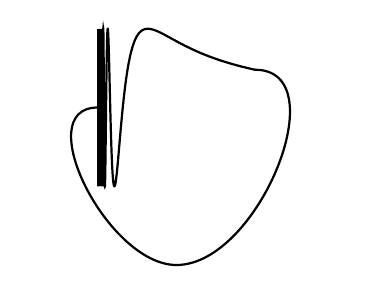
\begin{tikzpicture}
    \draw[thick] plot[domain=0.01:2,samples=5000] (\x,{sin(1/\x r)});
    \draw[thick] (0,1) -- (0,-1);
    \draw[thick] (2,{sin(0.5 r)}) to[out=0, in=0] (1,-2) to[out=180, in=180] (0,0);
  \end{tikzpicture}
  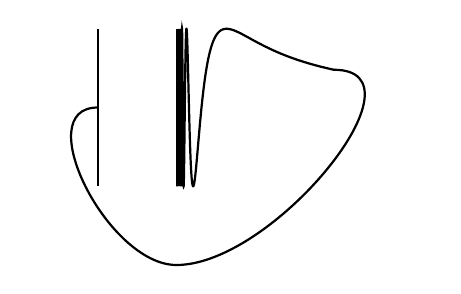
\begin{tikzpicture}
    \draw[thick] plot[domain=0.01:2,samples=5000] (\x,{sin(1/\x r)});
    \draw[thick] (-1,1) -- (-1,-1);
    \draw[thick] (2,{sin(0.5 r)}) to[out=0, in=0] (0,-2) to[out=180, in=180] (-1,0);
  \end{tikzpicture}
  \caption{The Warsaw circle and the separated Warsaw circle}
  \label{fig:Warsaw-circle}
\end{figure}
\end{exmp}

We conclude that sheaf cohomology gives the `best answer':
\begin{itemize}
\item The Eilenberg--MacLane approach works for spaces with many maps out of it (paracompact Hausdorff).
\item Singular cohomology works for spaces with many maps into it (CW-complexes).
\item De Rham cohomology works for manifolds (what we might call locally trivial spaces?).
\end{itemize}

The introduction of \citeauthor{lurieInfinityTopoi2003}'s preprint \citetitle{lurieInfinityTopoi2003}~\cite{lurieInfinityTopoi2003} also discusses these various notions of cohomology; we recommend taking a look.
The next section discusses the novel ideas from Lurie's work.

\section{Stacks and higher topoi}
The goal of \citeauthor{lurieInfinityTopoi2003}'s preprint \citetitle{lurieInfinityTopoi2003}~\cite{lurieInfinityTopoi2003} was to generalise the set \([X,K(G,n)]\) of homotopy classes of maps into an Eilenberg--MacLane space to the set \([X,Y]\) of homotopy classes of maps into an arbitrary space/homotopy type/Kan complex/\oo-groupoid/anima\footnote{These words all mean the same thing: they are presentations of topological spaces up to weak homotopy equivalence. When we say `space' in this section, this is what we mean, and we always use the adjective `topological' when talking about topological spaces. If \(Y\) is a Kan complex, then \([X,Y]\) should be interpreted as the set \([X,\abs{Y}]\) of homotopy classes of maps into the geometric realisaton of \(Y\).} \(Y\), using an `internal' definition in terms of sheaves on \(X\).

\begin{defn}
A \emph{sheaf of spaces} (also called an \emph{\oo-stack}) on a topological space \(X\) is a functor
\[ \mathcal F\colon\open(X)\opp\to\catSpace \]
into the \oo-category of spaces (often also denoted \(\mathcal S\)) such that for every open cover \(U=\bigcup_{i\in I}U_i\), the diagram
\begin{equation*}
  \begin{tikzcd}[column sep=small]
    \mathcal F(U) \ar{r} & \prod\limits_{i_0\in I}\mathcal F(U_{i_0}) \ar[shift left]{r} \ar[shift right]{r} & \prod\limits_{i_0,i_1\in I}\mathcal F(U_{i_0}\cap U_{i_1}) \ar[shift left=2]{r} \ar{r} \ar[shift right=2]{r} & \prod\limits_{i_0,i_1,i_2\in I}\mathcal F(U_{i_0}\cap U_{i_1}\cap U_{i_2}) \ar[shift left=3]{r} \ar[shift left]{r} \ar[shift right]{r} \ar[shift right=3]{r} & \ldots
  \end{tikzcd}
\end{equation*}
realises \(\mathcal F(U)\) as the homotopy limit (the limit in the \(\infty\)-categorical sense~\cite[Definition 1.2.13.4]{lurieHigherToposTheory2009}) of the rest of the diagram.
\end{defn}

If we work with the \oo-category \(\catSpace_{\leq n}\) of \(n\)-truncated spaces (that is, spaces with vanishing homotopy groups above degree \(n\)), we only need to consider the diagram up to the \((n+1)\)-fold product.
For instance, for \(n=0\) we have \(\catSpace_{\leq 0}\simeq\catSet\), and we only need to look at the part
\begin{equation*}
  \begin{tikzcd}[column sep=small]
    \mathcal F(U) \ar{r} & \prod\limits_{i_0\in I}\mathcal F(U_{i_0}) \ar[shift left]{r} \ar[shift right]{r} & \prod\limits_{i_0,i_1\in I}\mathcal F(U_{i_0}\cap U_{i_1})
  \end{tikzcd}
\end{equation*}
as we indeed did before for sheaves of sets.
(This is related to the fact that \((-)^\sharp=\check{H}^0(X,\check{H}^0(X,-))\): after one iteration of \(\check{H}^0(X,-)\), the map from \(\mathcal F(U)\) to the equaliser of \(\prod_i\mathcal F(U_i)\rightrightarrows \prod_{i,j}\mathcal F(U_i\cap U_j)\) is \((-1)\)-truncated (that is, injective).
After the second iteration, it is \((-2)\)-truncated, so an isomorphism.)

The \oo-category of \(n\)-truncated spaces can alternatively be presented as the \oo-category of \(n\)-groupoids (for \(n\geq -2\)).
In the low degrees, the \oo-category of \((-2)\)-groupoids is equivalent to the terminal category; the \oo-category of \((-1)\)-groupoids is equivalent to the walking arrow category \(\initial\to\terminal\); and the \oo-category is equivalent o the category of sets.

\begin{exmp}
A sheaf of \(1\)-truncated spaces is a \emph{stack} (in \(1\)-groupoids): it is a functor \(\open(X)\opp\to\catGroupoid\) (as \oo-categories) with a gluing condition.
\end{exmp}

\begin{exmp}
The association
\[ U \mapsto \{\text{rank } n \text{ locally constant sheaves on } U\}^\cong \]
sending an open \(U\) to the groupoid core of the full subcategory of rank \(n\) locally constant sheaves is a stack.
It is the constant sheaf \(\deloop\GL_n(\underline{\bb Z})\).
The sheaf condition says: if we have a family \((\mathcal G_i)_{i\in I}\) of locally constant sheaves and isomorphisms \((\phi_{ij}\colon\mathcal G_j|_{U_i\cap U_j}\cong\mathcal G_i|_{U_i\cap U_j})_{i,j\in I}\) such that \(\phi_{ij}|_{U_i\cap U_j\cap U_k}\circ\phi_{jk}|_{U_i\cap U_j\cap U_k}=\phi_{ik}|_{U_i\cap U_j\cap U_k}\), then we can glue the \(\mathcal G_i\) to a sheaf \(\mathcal G\) on \(U\) -- this is just `gluing sheaves'!
\end{exmp}

\begin{rmk}
The classical literature about (\(1\)-)stacks translates everything in concrete statements about \(1\)-categories.
\end{rmk}

\begin{thm}[name={\cite[Theorem~7.1.0.1]{lurieHigherToposTheory2009}}]
If \(X\) is a paracompact topological space and \(K\) is a space, then the functor
\[ \rightderived\Gamma(X,-)\colon\catSheaf(X,\catSpace)\to\catSheaf(*,\catSpace) \simeq\catSpace \]
induced by \(X\to *\) satisfies
\[ \pi_0\rightderived\Gamma(X,\underline{K}) \cong [X,K]\text{.} \]
\end{thm}
The proof of this theorem is finished on page~705 of \cite{lurieHigherToposTheory2009}.

\section{Relative Poincaré duality}
\todo{write}

\remyquote{Should we go back to earth?}

%%% Local Variables:
%%% mode: latex
%%% TeX-master: "../main"
%%% End:
